\section{Usability}
\label{sec:usability}

Before setting up and using the Safeplug device, we read a variety of news articles as well as opinions through the Tor mailing list~\cite{tormailinglist}.  There were many thoughts on the Terms of Service and the option to use the device as a Tor relay node; this inspired us to start our analysis with these items.  

\subsection{Terms of Service}
\label{tos}
Safeplug's Terms of Service are interesting because they are controlling, yet the product they are for is a device for anonymization.  The first section of the Terms of Service explains how to agree to them:

\begin{quotation}
``You must agree to these TOS before you can use the Service. You can agree to these TOS by: a) actually using the Service, or b) clicking a box that indicates you agree to the Service, where such a box is made available to you.'' \cite{safeplug}
\end{quotation}

This is worth noting because option b) described above did not exist in any part of the setup process for Safeplug.  The Terms of Service continues by notifying readers that Pogoplug can change them any time they wish:

\begin{quotation}
``Pogoplug may update or change these TOS from time to time and recommends that you review the TOS on a regular basis at www.pogoplug.com/safeplug. You understand and agree that your continued use of the Service after the TOS has changed constitutes your acceptance of the TOS as revised. '' \cite{safeplug}
\end{quotation}

Most Safeplug users will likely not read the Terms of Service once, let alone on a regular basis; therefore, most users will be blind to any changes.  It is also interesting that these Terms of Service are only accessible through a small link at the bottom of the Safeplug website \cite{safeplug}; specifically, there is no documentation, including the Terms of Service, in the package that the device was shipped in.  Further along in the Terms of Service, the makers of Safeplug were sloppy when they wrote:

\begin{quotation}
``Pogoplug includes several open source components in the Software. You agree to abide by the terms of the relevant licenses, as may be updated by Pogoplug from time to time at http://pogoplug.com/home-en-developers-open-source.html. '' \cite{safeplug}
\end{quotation}

The link included is a dead link and takes the user to a web page with a 404 error.  This lack of attention to detail or respect for open source licenses does not put Pogoplug in a good light.  In fact, the Tor mailing list noted this particularly, since Tor is an open source project \cite{tormailinglist}.  The last section of the Terms of Service that stood out described Pogoplug's policy on updates:

\begin{quotation}
``As part of the Service, you may from time to time receive updates to the Software from Pogoplug that may be automatically downloaded and installed to your applicable device. These updates may include bug fixes, security enhancements or improvements, or entirely new versions of the Software. You agree that Pogoplug may automatically deliver such updates to you as part of the Service. '' \cite{safeplug}
\end{quotation}

This should raise a red flag for users because they may not know when the software in their device is being changed or what it is changing to.  While Safeplug makes many claims about providing anonymity, users are simply putting their trust in a different entity, namely Pogoplug.

\subsection{Tor Relay Node Option}
One of Safeplug's configurations is the use of the device as a Tor relay node in the Tor network.  When the device is initially setup, the default setting is to not use it as a relay node.  

One of our concerns is how understandable this setting is to the average Internet user.  The settings page describes Tor in an extremely basic way, as shown in Figure~\ref{fig:funnydesc}, but describes the functionality of a Tor relay node in a much more technical manner.  This description is shown in Figure~\ref{fig:relaydesc}.  If the majority of users can only understand the simpler description, then they likely won't understand the description of a Tor relay node.  This could be a problem if users simply decide not to do anything with that setting (i.e. don't change the setting to use Safeplug as a relay node).  Then there would be a large increase in use of the Tor network, yet most of the users are not giving back to it.

\begin{figure}[th]
\begin{center}
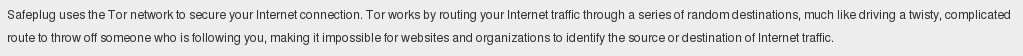
\includegraphics[width=\textwidth]{funnydesc.png}
\caption{Description of Tor on Safeplug settings page.}
\label{fig:funnydesc}
\end{center}
\end{figure}

\begin{figure}[th]
\begin{center}
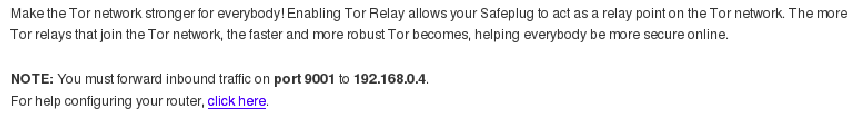
\includegraphics[width=\textwidth]{relaydesc.png}
\caption{Description of a Tor relay on Safeplug settings page.}
\label{fig:relaydesc}
\end{center}
\end{figure}

This could easily be remedied; Safeplug should choose a target audience and have consistent descriptions.  The best option is to explain the Tor network and the functionality of a Tor relay node at the same level, preferably a level that normal Internet users can understand.  This increases the chances that users will run their Safeplug as a relay node.

\subsection{Internet Use}
\label{inetuse}

\subsubsection{Setting up Safeplug} The first step was to plug Safeplug into our router and activate our device.  Our instructions are shown in Figure~\ref{fig:instructions}.  We followed them, activated our device, and then ended on the configuration page.  The configuration page has a combination of platforms and browsers, with a different set of proxy configuration instructions for each one.  It is interesting to note that the only platform options were: OSX, Windows, Android, and iOS.  Figure~\ref{fig:proxyconfig} shows our configuration. 

\begin{figure}[t]
\begin{center}
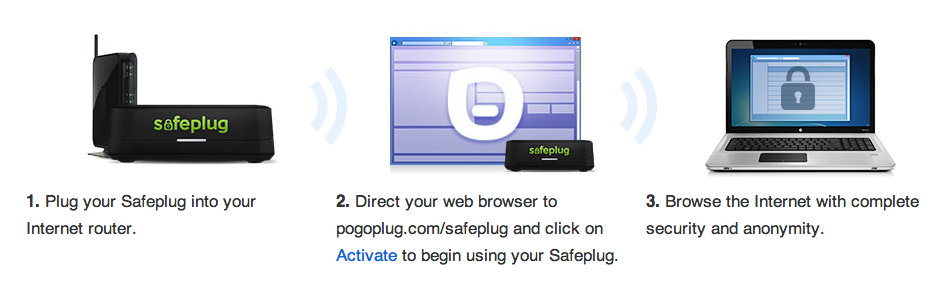
\includegraphics[width=.75\textwidth]{instructions}
\caption{Configuration instructions.}
\label{fig:instructions}
\end{center}
\end{figure}

\begin{figure}[t]
\begin{center}
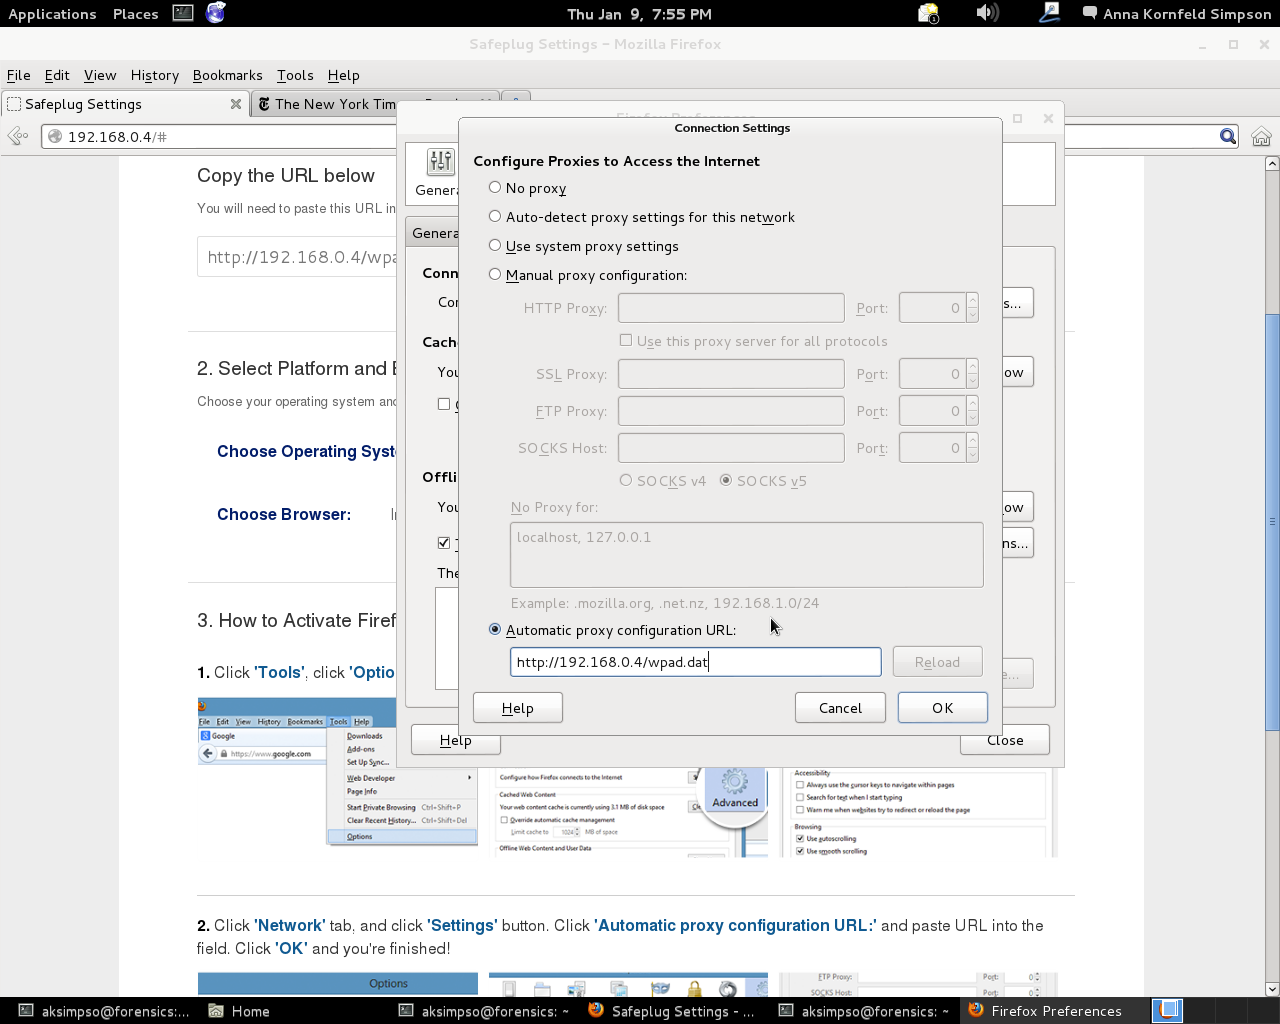
\includegraphics[width=.75\textwidth]{proxyconfig}
\caption{Proxy Configuration.}
\label{fig:proxyconfig}
\end{center}
\end{figure}

After we finished our configuration, we were taken to our settings.  This page is shown in Figure~\ref{fig:settings}.  This allowed us to turn on/off Tor, add whitelisted websites, turn on/off ad-blocking, and turn on/off the ability of our device to be a relay node.  

\begin{figure}[htb]
\begin{center}
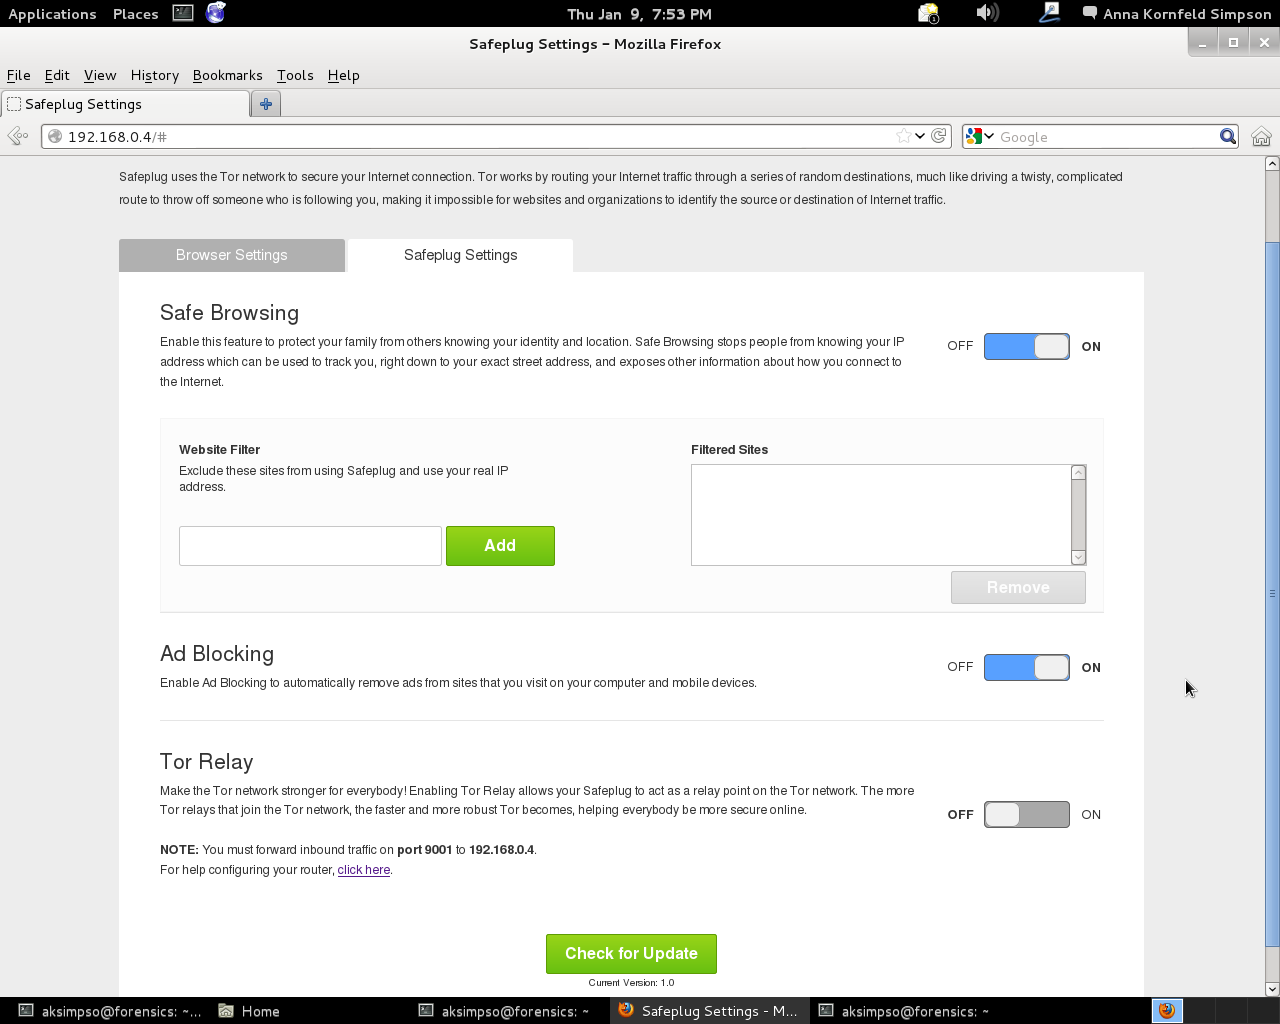
\includegraphics[width=.75\textwidth]{settings}
\caption{Settings page.}
\label{fig:settings}
\end{center}
\end{figure}

\subsubsection{Using the Internet} Figure~\ref{fig:before} shows what a web page looks like before turning Tor and ad-blocking on, while Figure~\ref{fig:after} shows the same website after turning Tor and ad-blocking on.  Both of these figures show our IP address in the top right corner; due to the change in IP address we can see that our traffic is being routed through Tor.  

\begin{figure}[htb]
\centering
\begin{subfigure}[b]{.4\textwidth}
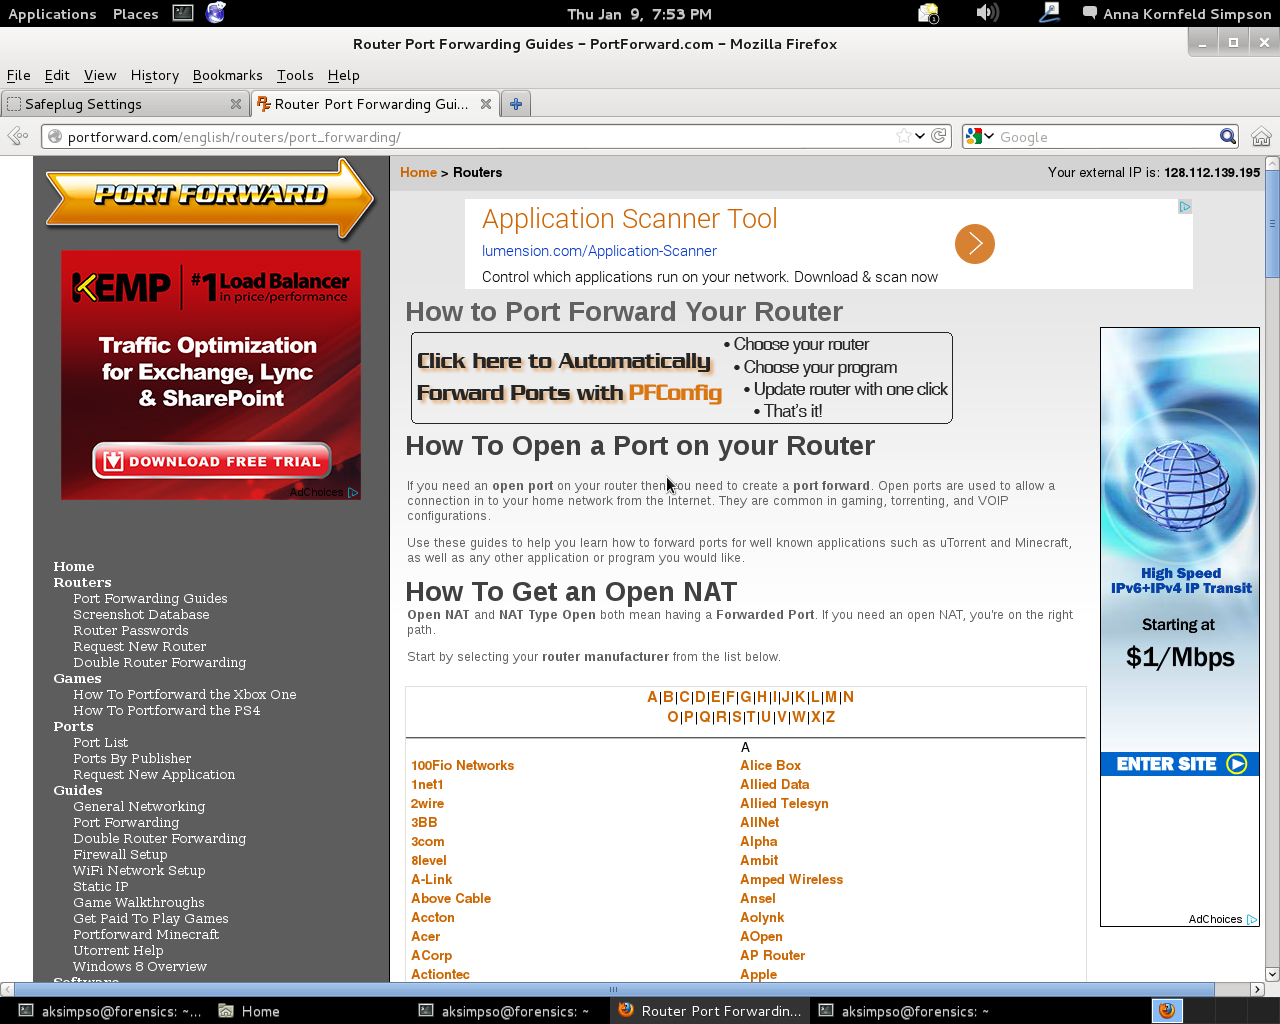
\includegraphics[width=\textwidth]{before}
\caption{Web page before using Tor and ad-blocking.}
\label{fig:before}
\end{subfigure}%
\quad
\begin{subfigure}[b]{.4\textwidth}
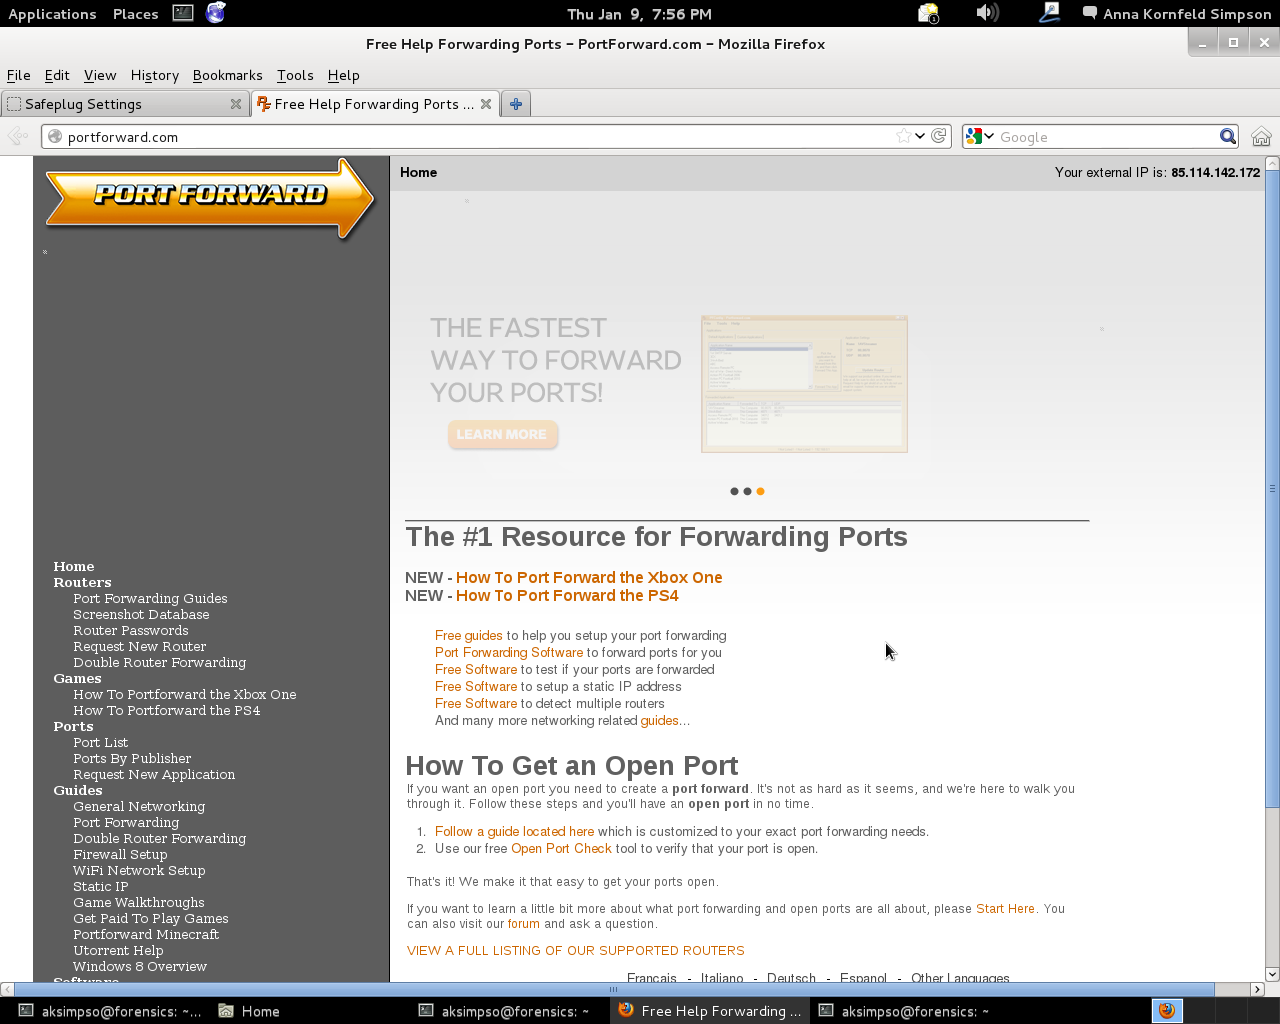
\includegraphics[width=\textwidth]{after}
\caption{Web page after using Tor and ad-blocking.}
\label{fig:after}
\end{subfigure}
\end{figure}

Next, we wanted to see how usable this would be to a normal Internet user.  A user would probably decide not to use Safeplug if they couldn't read their web pages (if they weren't in their native language), or if they couldn't log into their accounts (some web sites will lock a user out if they try to login from multiple countries in a short time period).  While browsing the Internet, we experienced some pages in German and Swedish, which is expected with Tor; if a user is not familiar with Tor, then they may just get frustrated and stop using Safeplug altogether.  We were also prompted with the page in Figure~\ref{fig:funnygoogle} when we tried to log into our Google account. 

\begin{figure}[htb]
\begin{center}
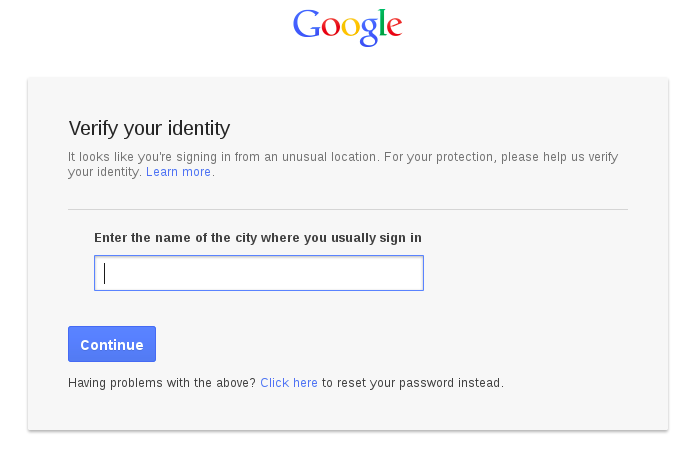
\includegraphics[width=0.5\textwidth]{funnygoogle}
\caption{Google's response after trying to log in.}
\label{fig:funnygoogle}
\end{center}
\end{figure}

\subsection{Cookies}  While browsing the Internet, we logged into a Google Account in a tab, and then subsequently went to a website that had the Google+ logo in a different tab.  When we clicked on the Google+ logo, it remember who we are; so we can confirm that we still have first-party cookies.  We experienced the same situation with Facebook and its corresponding ``like'' button.

This is clearly not the perfect ``anonymity'' that Safeplug promised in their publicity.  Although normal use does follow this model of persisting logins across browser tabs and sessions, a user concerned about anonymity and seeing each session coming up differently (German vs Swedish) might mistakenly believe that they do not have to log out of their social media accounts to preserve their anonymity when accessing other websites.

More interesting and damaging to the user's control over their anonymity would be third-party cookies because the user cannot remove those just by logging out.  It requires a trip to the browser settings to clear cookies (or not have them set in the first place).  We used the FourthParty plugin developed by Jonathan Mayer at Stanford to collect information about cookies and other browsing data during the client's use of the Safeplug \cite{fourthparty}.  When collecting data on the existence of third-party cookies, we analyzed two separate browsing sessions; they were both new sessions with no cookies.  One of the sessions used the ad-block feature of the Safeplug and the other did not.  After analyzing data from Fourthparty, we found many third-party cookies in both sessions.  These included cookies from: abmr.net, bizographics.com, krxd.net, and bluekai.com among many others.
